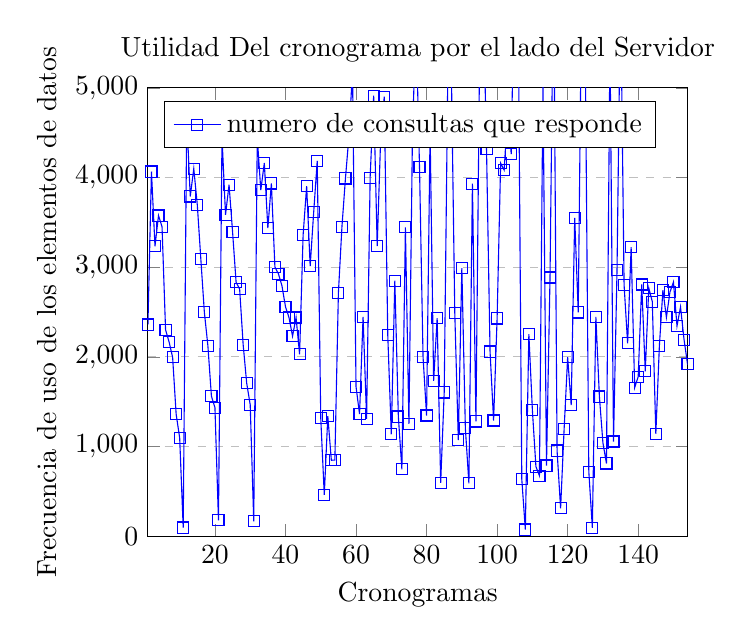
\begin{tikzpicture}
\begin{axis}[
    title={Utilidad Del cronograma por el lado del Servidor},
    xlabel={Cronogramas},
    ylabel={Frecuencia de uso de los elementos de datos},
    xmin=1, xmax=154,
    ymin=0, ymax=5000,
    xtick={},
    ytick={},
    legend pos=north west,
    ymajorgrids=true,
    grid style=dashed,
]

\addplot[
    color=blue,
    mark=square,
    ]
    coordinates {
%UTILIDAD TOTAL
%(cronograma, numero cues que usan al cronograma)
(1,2360)
(2,4067)
(3,3234)
(4,3576)
(5,3451)
(6,2302)
(7,2166)
(8,1996)
(9,1361)
(10,1097)
(11,96)
(12,4669)
(13,3789)
(14,4099)
(15,3694)
(16,3091)
(17,2497)
(18,2124)
(19,1562)
(20,1434)
(21,177)
(22,4452)
(23,3585)
(24,3919)
(25,3393)
(26,2831)
(27,2757)
(28,2136)
(29,1707)
(30,1465)
(31,166)
(32,4445)
(33,3859)
(34,4162)
(35,3435)
(36,3934)
(37,3003)
(38,2926)
(39,2793)
(40,2559)
(41,2438)
(42,2231)
(43,2439)
(44,2028)
(45,3359)
(46,3904)
(47,3012)
(48,3615)
(49,4185)
(50,1316)
(51,460)
(52,1339)
(53,847)
(54,849)
(55,2711)
(56,3447)
(57,3990)
(58,4465)
(59,5194)
(60,1668)
(61,1361)
(62,2447)
(63,1309)
(64,3999)
(65,4912)
(66,3235)
(67,4455)
(68,4902)
(69,2242)
(70,1137)
(71,2850)
(72,1334)
(73,746)
(74,3444)
(75,1253)
(76,4486)
(77,5749)
(78,4116)
(79,2001)
(80,1346)
(81,4520)
(82,1731)
(83,2433)
(84,596)
(85,1603)
(86,5087)
(87,5285)
(88,2492)
(89,1072)
(90,2990)
(91,1203)
(92,590)
(93,3932)
(94,1280)
(95,5239)
(96,6100)
(97,4318)
(98,2059)
(99,1290)
(100,2428)
(101,4161)
(102,4083)
(103,4751)
(104,4262)
(105,6535)
(106,5770)
(107,634)
(108,74)
(109,2254)
(110,1407)
(111,776)
(112,675)
(113,5041)
(114,788)
(115,2885)
(116,6394)
(117,955)
(118,310)
(119,1196)
(120,1996)
(121,1462)
(122,3551)
(123,2495)
(124,6246)
(125,5397)
(126,720)
(127,94)
(128,2445)
(129,1557)
(130,1041)
(131,811)
(132,5520)
(133,1056)
(134,2973)
(135,6148)
(136,2802)
(137,2151)
(138,3225)
(139,1657)
(140,1779)
(141,2807)
(142,1839)
(143,2768)
(144,2616)
(145,1141)
(146,2117)
(147,2744)
(148,2440)
(149,2722)
(150,2835)
(151,2344)
(152,2557)
(153,2192)
(154,1916)
(155,1913)
(156,2171)
    };
    \legend{numero de consultas que responde}

\end{axis}
\end{tikzpicture}

